\usetikzlibrary{arrows,positioning}
	
\section{Planung und Organisation}
	
\subsection{Projektorganisation}
An dem Projekt werden folgende Personen mitarbeiten:
\\\\
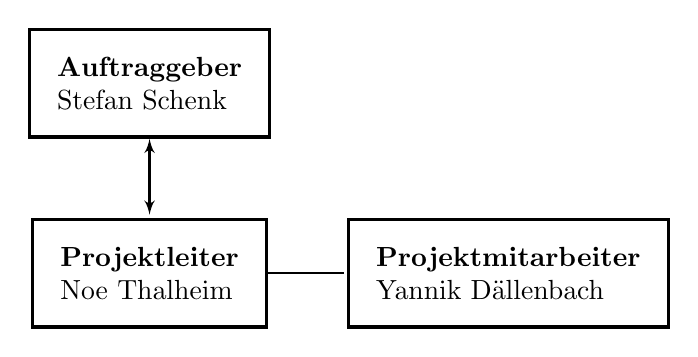
\begin{tikzpicture}[node distance=1cm, auto]  
\tikzset{
	    mynode/.style={rectangle,align=left,draw=black, top color=white, bottom color=white!50,very thick, inner sep=1em, minimum size=3em, text centered},
	    myarrow/.style={->, >=latex', shorten >=1pt, thick},
	    mylabel/.style={text width=7em, text centered} 
	}  
	\node[mynode] (auftraggeber) {\textbf{Auftraggeber}\\Stefan Schenk};  
	\node[mynode, below=1cm of auftraggeber] (projektleiter) {\textbf{Projektleiter}\\Noe Thalheim};  
	\node[mynode, right=of projektleiter] (projektmitarbeiter1) {\textbf{Projektmitarbeiter}\\Yannik Dällenbach};


	\draw[myarrow] [<->] (auftraggeber.south) -- (projektleiter.north);	
	\draw[myarrow] [-] (projektleiter.east) -- (projektmitarbeiter1.west);

	\end{tikzpicture} 
	\medskip

	Die Aufgabenverteilung wird das ganze Projekt gleich bleiben.
	
	\subsection{Termine}
	
	Für unser Projekt sind folgende Termine von Wichtigkeit:
	\begin{description}
		\item[] Starttermin: 05.02.2013
		\item[] Endtermin: 04.06.2013
	\end{description}
	Daraus ergibt sich für unser Projekt folgender Terminplan:
	\\ \\
	\tiny{
	\begin{tabular}{| p{2cm} | p{1cm} | p{1cm} | p{1cm} | p{1cm} | p{1cm} | p{1cm} |}
	\hline
	\rowcolor[gray]{0.9}  & 12.02.13 - 19.02.13 & 19.02.13 - 05.03.13 & 5.03.13 - 19.03.13 & 19.03.13 - 07.05.13 & 7.05.13 - 21.05.13 & 21.05.13 - 04.06.13 \\
	\hline
	Initialisierung & \cellcolor{yellow} & & & & & \\
	\hline
	Voranalyse & &  \cellcolor{yellow}& & & & \\
	\hline
	Konzept & & &  \cellcolor{yellow}& & & \\
	\hline
	Realisierung & & & &  \cellcolor{yellow}& & \\
	\hline
	Einführung & & & & & \cellcolor{yellow}& \\
	\hline
	Abschluss & & & & &  &\cellcolor{yellow} \\
	\hline
	\end{tabular}	
	}
	\small{
	\subsection{Prioritäten}
	Unsere Prioritäten für dieses Projekt sind das Verstehen und Implementieren von Evolutionären Algorithmen und somit das Selbststudium in diesen Gebieten. Zudem ist es uns wichtig durch dieses Projekt Erfahrungen im Zusammenhang mit der Programmierung in Objective-C sammeln zu können. 
}